\documentclass[10pt,twocolumn,letterpaper]{article}

\usepackage{cvpr}
\usepackage{float}
\usepackage{times}
\usepackage{epsfig}
\usepackage{graphicx}
\usepackage{amsmath}
\usepackage{amssymb}
\usepackage{subcaption}

% Include other packages here, before hyperref.

% If you comment hyperref and then uncomment it, you should delete
% egpaper.aux before re-running latex.  (Or just hit 'q' on the first latex
% run, let it finish, and you should be clear).
\usepackage[breaklinks=true,bookmarks=false]{hyperref}

\cvprfinalcopy

\def\cvprPaperID{****} % *** Enter the CVPR Paper ID here
\def\httilde{\mbox{\tt\raisebox{-.5ex}{\symbol{126}}}}

% Pages are numbered in submission mode, and unnumbered in camera-ready
%\ifcvprfinal\pagestyle{empty}\fi
\setcounter{page}{1}
\begin{document}

%%%%%%%%% TITLE
\title{
    Super Convergence: Very Fast Training of Residual Networks Using Large
    Learning Rates\\
    \large ICLR Reproducibility Challenge}

\author{Keivaun Waugh\\
University of Texas at Austin\\
{\tt\small keivaunwaugh@gmail.com}
% For a paper whose authors are all at the same institution,
% omit the following lines up until the closing ``}''.
% Additional authors and addresses can be added with ``\and'',
% just like the second author.
% To save space, use either the email address or home page, not both
\and
Paul Choi\\
University of Texas at Austin\\
{\tt\small choipaul96@gmail.com}
}

\maketitle
%\thispagestyle{empty}

%%%%%%%%% ABSTRACT
\begin{abstract}
In this paper, we aim to evaluate the reproducibility of the experiments
    detailed in the paper ``Super-Convergence: Very Fast Training of Residual
    Networks Using Large Learning Rates'' \cite{SuperConvergence}
\end{abstract}

%%%%%%%%% BODY TEXT
\section{Introduction}
In an ICLR 2018 submission, the anonymous authors of \cite{SuperConvergence}
show that under certain training conditions, a phenomenon called
``super-convergence'' can be achieved, where ResNets \cite{ResNet} can be
trained an order of magnitude more quickly than when using normal training
methods.  Super-convergence simply requires using a cyclical learning rate
(CLR) versus the standard piecewise constant learning rate (PCLR). When using
the CLR method, the learning rate is slowly increased from a minimum learning
rate to a maximum learning rate, then slowly decreased back to the minimum
learning rate again, after which training stops. The number of iterations taken
to go from the minimum learning rate to the maximum and vice versa is referred
to as the step-size and is a hyperparameter.

The authors run a variety of experiments to see under what circumstances
super-convergence can be achieved with the CLR method. Using Cifar-10 and
Cifar-100 \cite{Cifar}, ImageNet \cite{ImageNet} and a variety of network
architectures, they were only able to induce super-convergence on Cifar-10 and
Cifar-100 using ResNet, and not at all on ImageNet.

There is still a significant amount of work to be done on investigating
super-convergence. It is still unclear when it can occur and if it can be
induced in a deterministic manner in other circumstances. In this paper we
investigate the current known quantities of super-convergence and attempt to
reproduce them.

\subsection{Target Questions}
We seek to reproduce the key experiments in \cite{SuperConvergence} and confirm
most significant claims made by the authors. Specifically, we aim to:
\begin{itemize}
    \item Confirm the existence of the super-convergence phenomenon
    \item Verify that super-convergence is superior to the PCLR method with
        limited training examples
    \item Verify the reported accuracy trends of using varying step sizes,
        learning rate ranges, and iterations for the CLR method
\end{itemize}
%------------------------------------------------------------------------------

\section{Method}
\label{sec:method}
Due to time and hardware constraints (lack of multiple GPUs), we were unable to
replicate all of the experiments that were listed in the paper. Therefore, we
had to choose which experiments from which we could glean the most. It was our
goal to show the existence or not of the following claims made in the paper.
Super-convergence:
\begin{itemize}
    \item allows the network to achieve higher test accuracy than traditional
        piece-wise constant learning rates (PCLR)
    \item requires an order of magnitude fewer iterations to converge than PCLR
    \item is more noticeable with fewer training examples
    \item works with various ResNet sizes
    \item works best with a certain step size
\end{itemize}

When available, we used the hyperparameters that the authors listed in their
paper. When these were omitted, we attempted to use standard values that are
used on Cifar-10 and ResNets.

\subsection{Implementation Details}
In the ICLR submitted paper, the authors mentioned that they would release
their code upon acceptance to the conference. However, upon Googling the paper
name, we found an arXiv version of the paper that links to the authors' source
code on GitHub. We chose to not look at this code and reimplement their
solution so that we could test the reproducibility under the information
that was listed in the ICLR paper.

As a starting point, we used the open source ResNet training on Cifar-10 code
available in the TensorFlow \cite{TensorFlow} repository. We modified the code
accordingly for each of the experiments.

A major limitation in our testing was our restriction to a single GPU for all
of the experiments. The authors stated that they used 8 Nvidia Titan Black
GPUs, which allowed them to test with batch sizes as large as 1536. We were
restricted to a batch size of 256. The authors found that increasing the batch
size significantly improved the performance of their CLR tests, so the
discrepancy between our results and the authors could be due to this. It was
unclear from the paper whether these large batch size were used with their PCLR
test as well.

%------------------------------------------------------------------------------

\section{Experiments}
All experiments were run on a single machine with a quad core Intel Core i5
processor, 16GB of RAM, and an Nvidia GTX 1070 GPU. The effect of batch sizes
on our results will be discussed in section \ref{sec:conclusion}.

\subsection{Existence of Super-Convergence}
\label{sec:existence_of_super_convergence}
Figure \ref{fig:clr_vs_pclr} shows the results we obtained when we ran the
tests displayed in figure 1a of the original paper. Here we can see from the
blue line that one of the CLR runs did peak and achieve better results than
PCLR with fewer iterations. However, the PCLR run achieved a higher final
accuracy on the test set, unlike what the authors reported. Additionally, the
CLR test was repeated with the same hyperparameters, but given the same number
of iterations as the PCLR test(green line). It achieved significantly worse
accuracy than the other two tests. Interestingly, the green run also had worse
accuracy than the blue run in the first ten thousand iterations, which suggests
that super-convergence is highly sensitive to the initial weight initialization
and the noise introduced by stochastic gradient descent.

\begin{figure*}[ht!]
    \begin{tabular}{cc}
        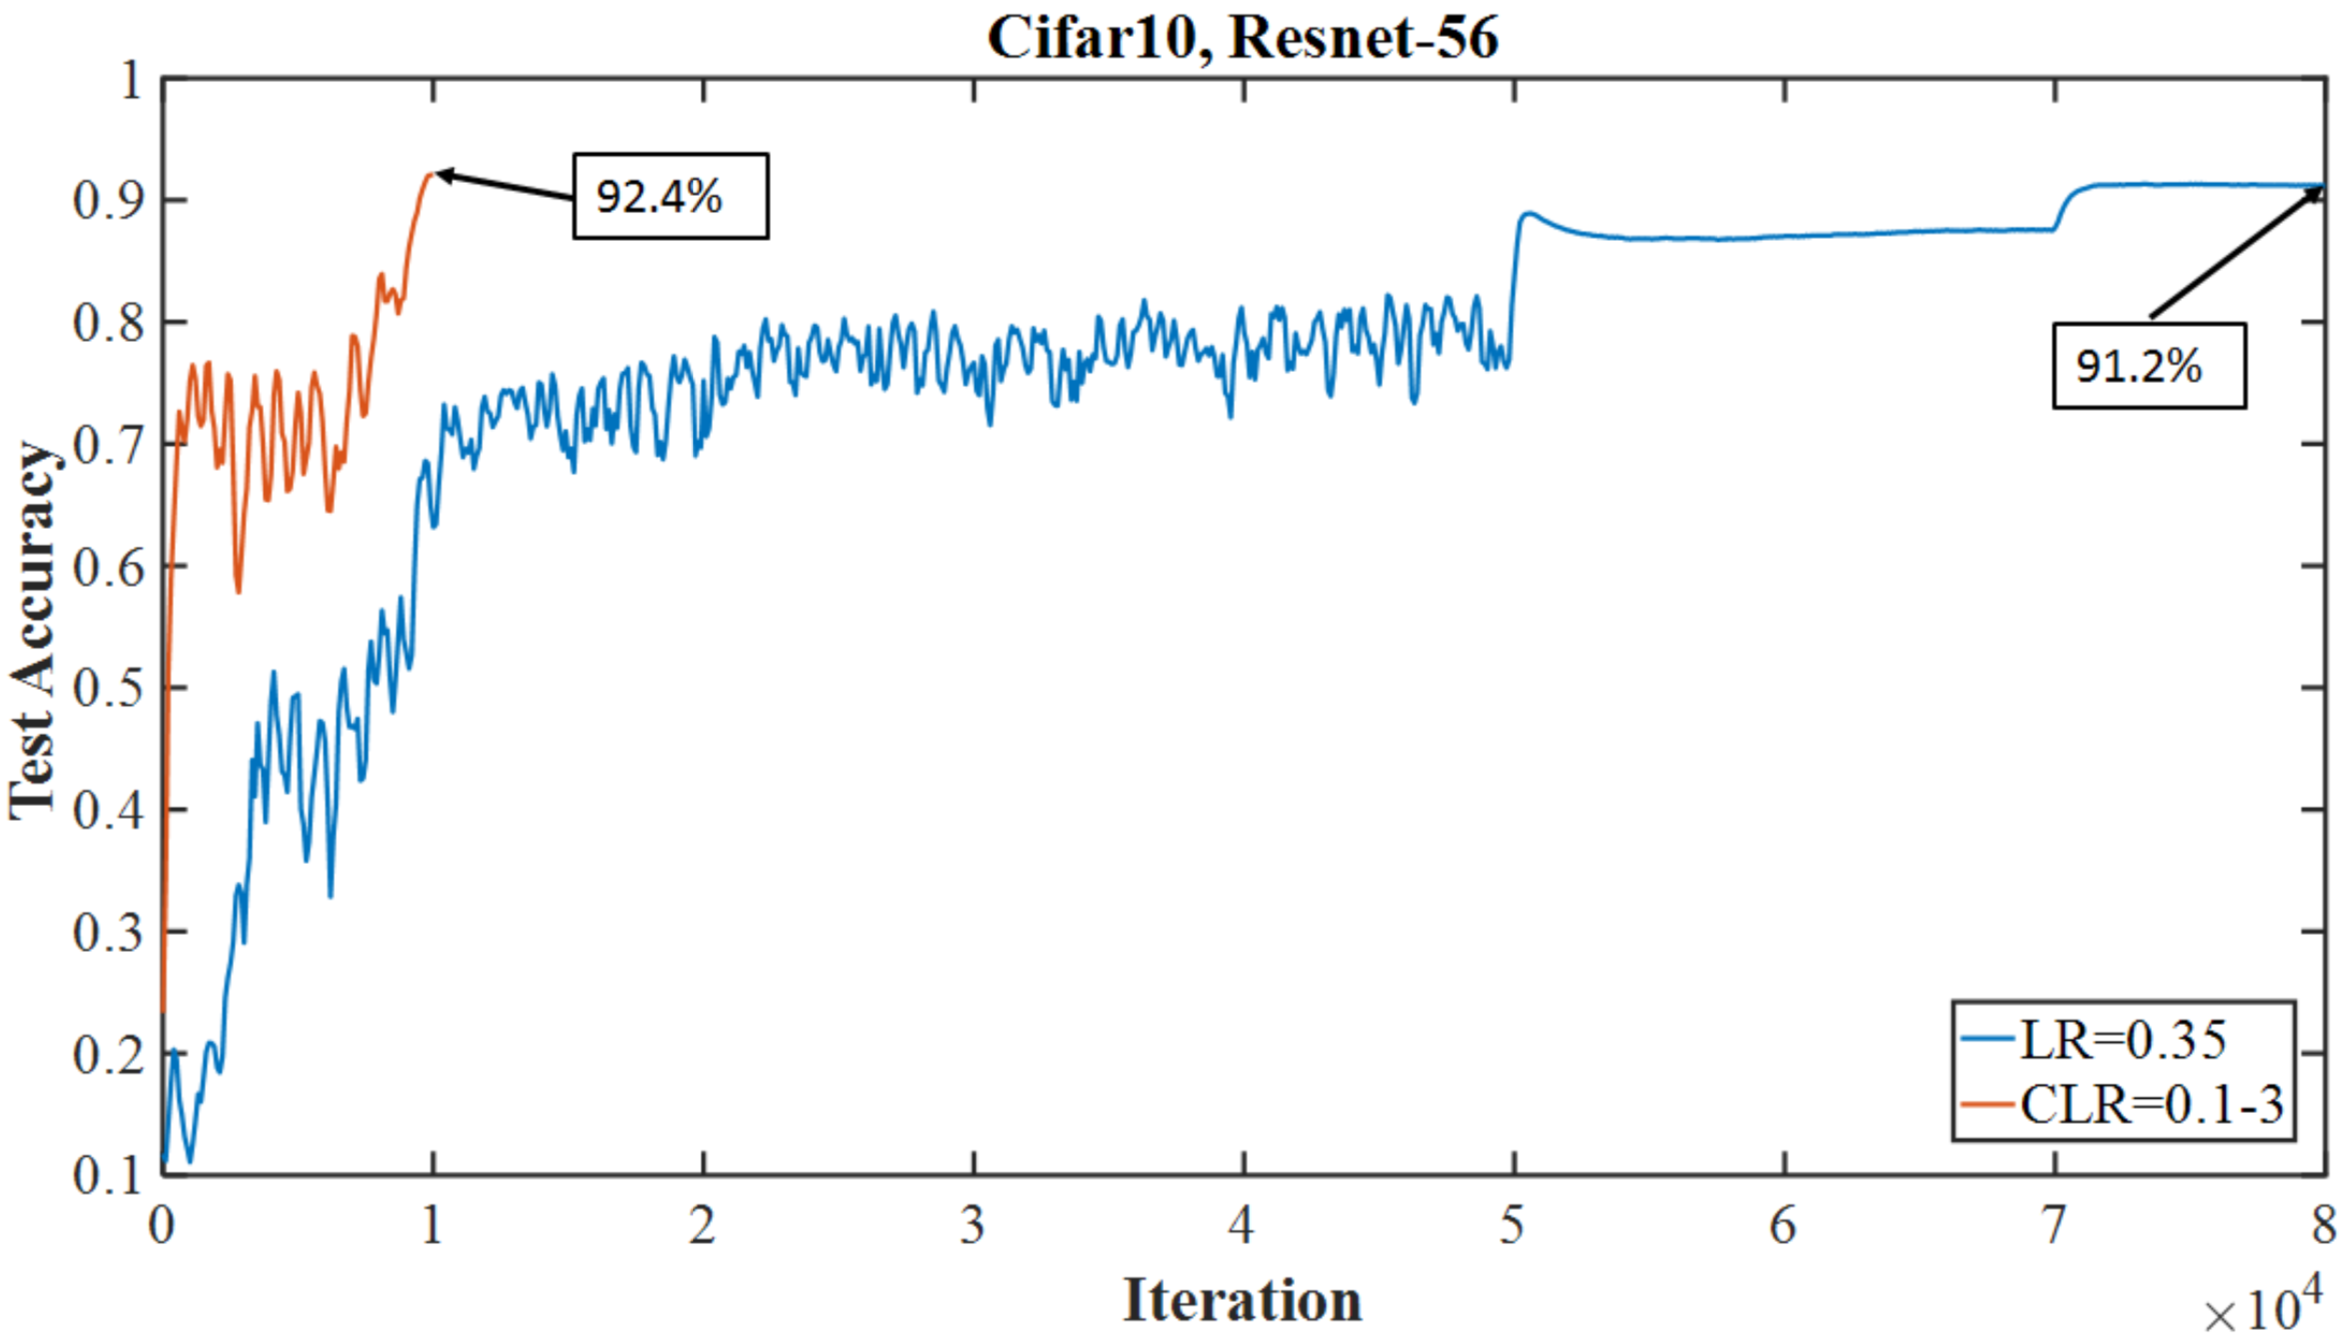
\includegraphics[trim=0 0 0 0, clip,
            width=3.25in]{images/figure_1a.png} &
        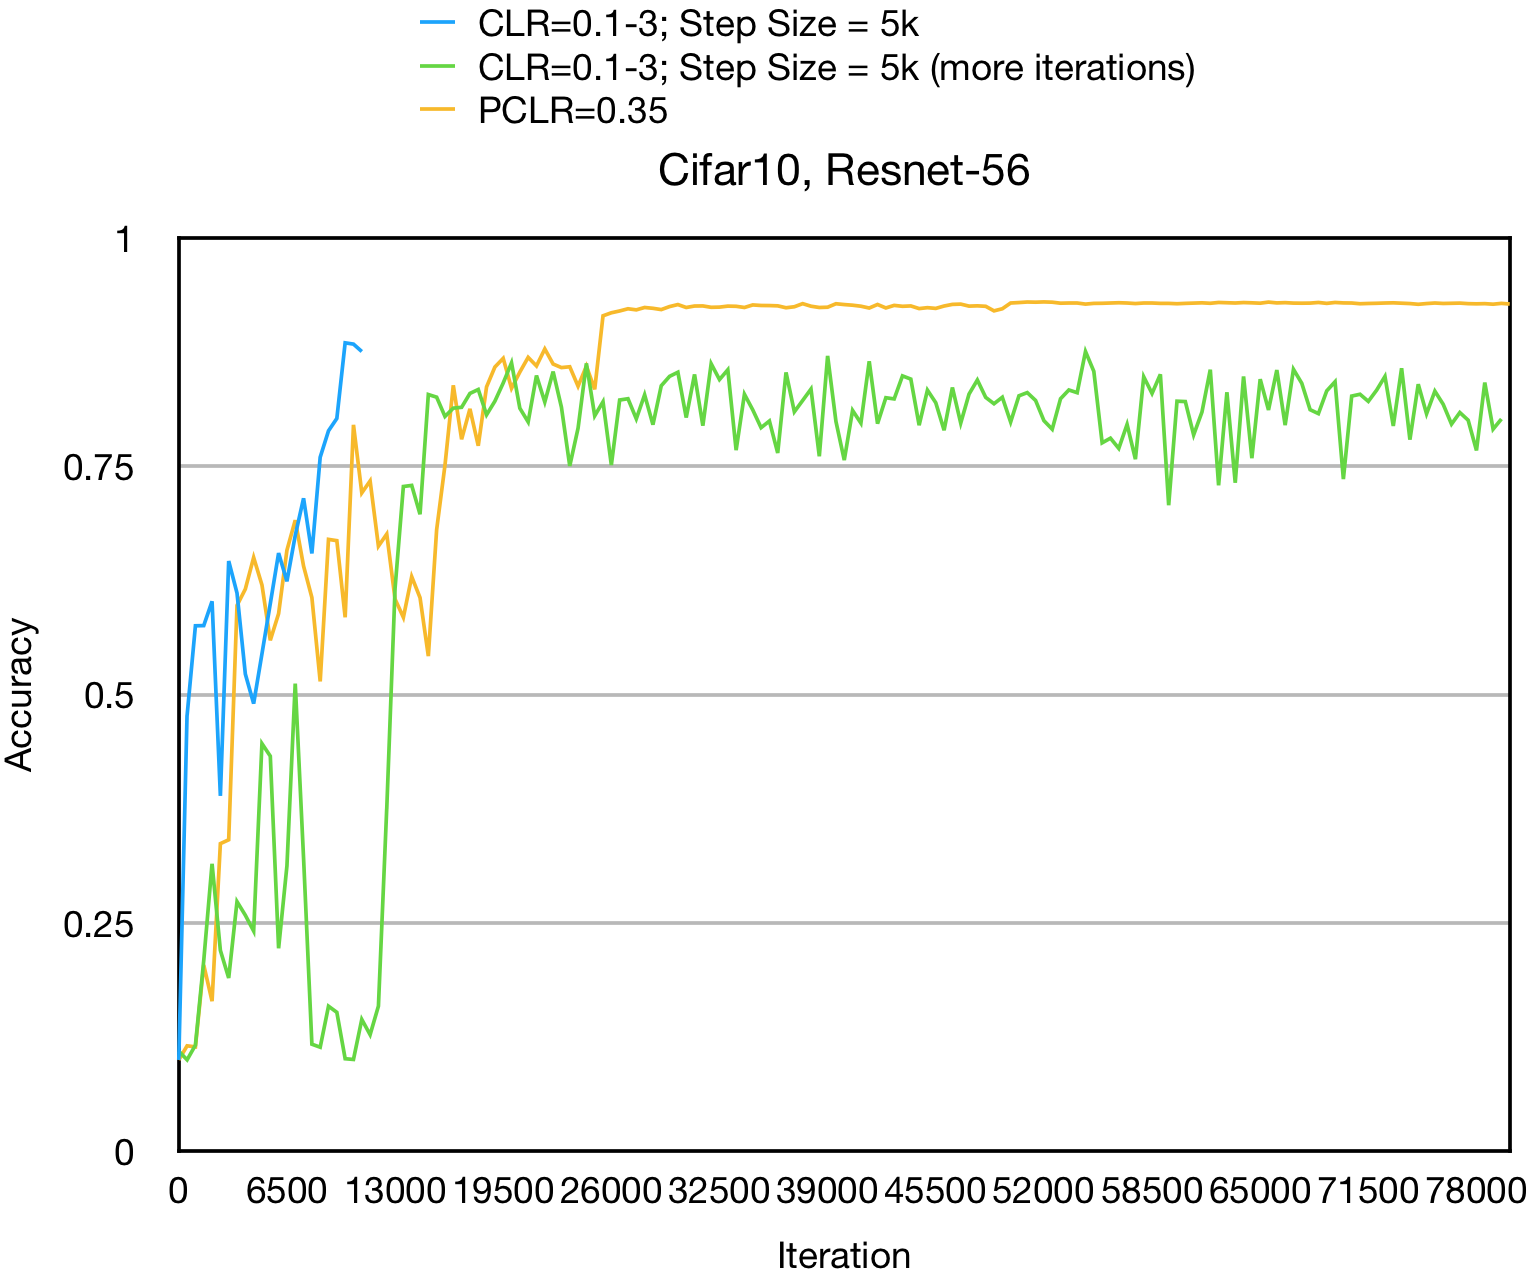
\includegraphics[trim=0 0 0 0, clip,
            width=3.25in]{images/clr_vs_pclr.png} \\
        Author's Results & Our Results \\
    \end{tabular}
    \caption{Cyclical learning rate (CLR) versus piecewise linear learning rate
    (LR/PCLR).}
    \label{fig:clr_vs_pclr}
\end{figure*}

\subsection{Effect of Step Size}
The authors ran experiments to determine the best step-size for CLR to achieve
the best super-convergence results.  Somewhat puzzling is the fact that the
authors display a step-size of three thousand appears to be better than five
thousand. However, they chose to use five thousand as their step-size in a
majority of their tests. Due to their description of CLR having only one
increasing LR phase and one decreasing LR phase, using a step-size of three
thousand would result in only six thousand total iterations needed to achieve
final peak accuracy. This would have decreased their required test time for
many of their experiments and would make the effect of super-convergence appear
more drastic as it would need $40\%$ fewer iterations than reported.

Our results for this experiment are listed in figure \ref{fig:step_size}. We
report similar trends in the step sizes, with accuracy increasing as step size
increases. However, as reported in section
\ref{sec:existence_of_super_convergence}, all of our accuracies are lower than
what the authors report. Even the trial with ten thousand step size has worse
performance than the traditional PCLR method.

\begin{figure*}[ht!]
    \begin{tabular}{cc}
        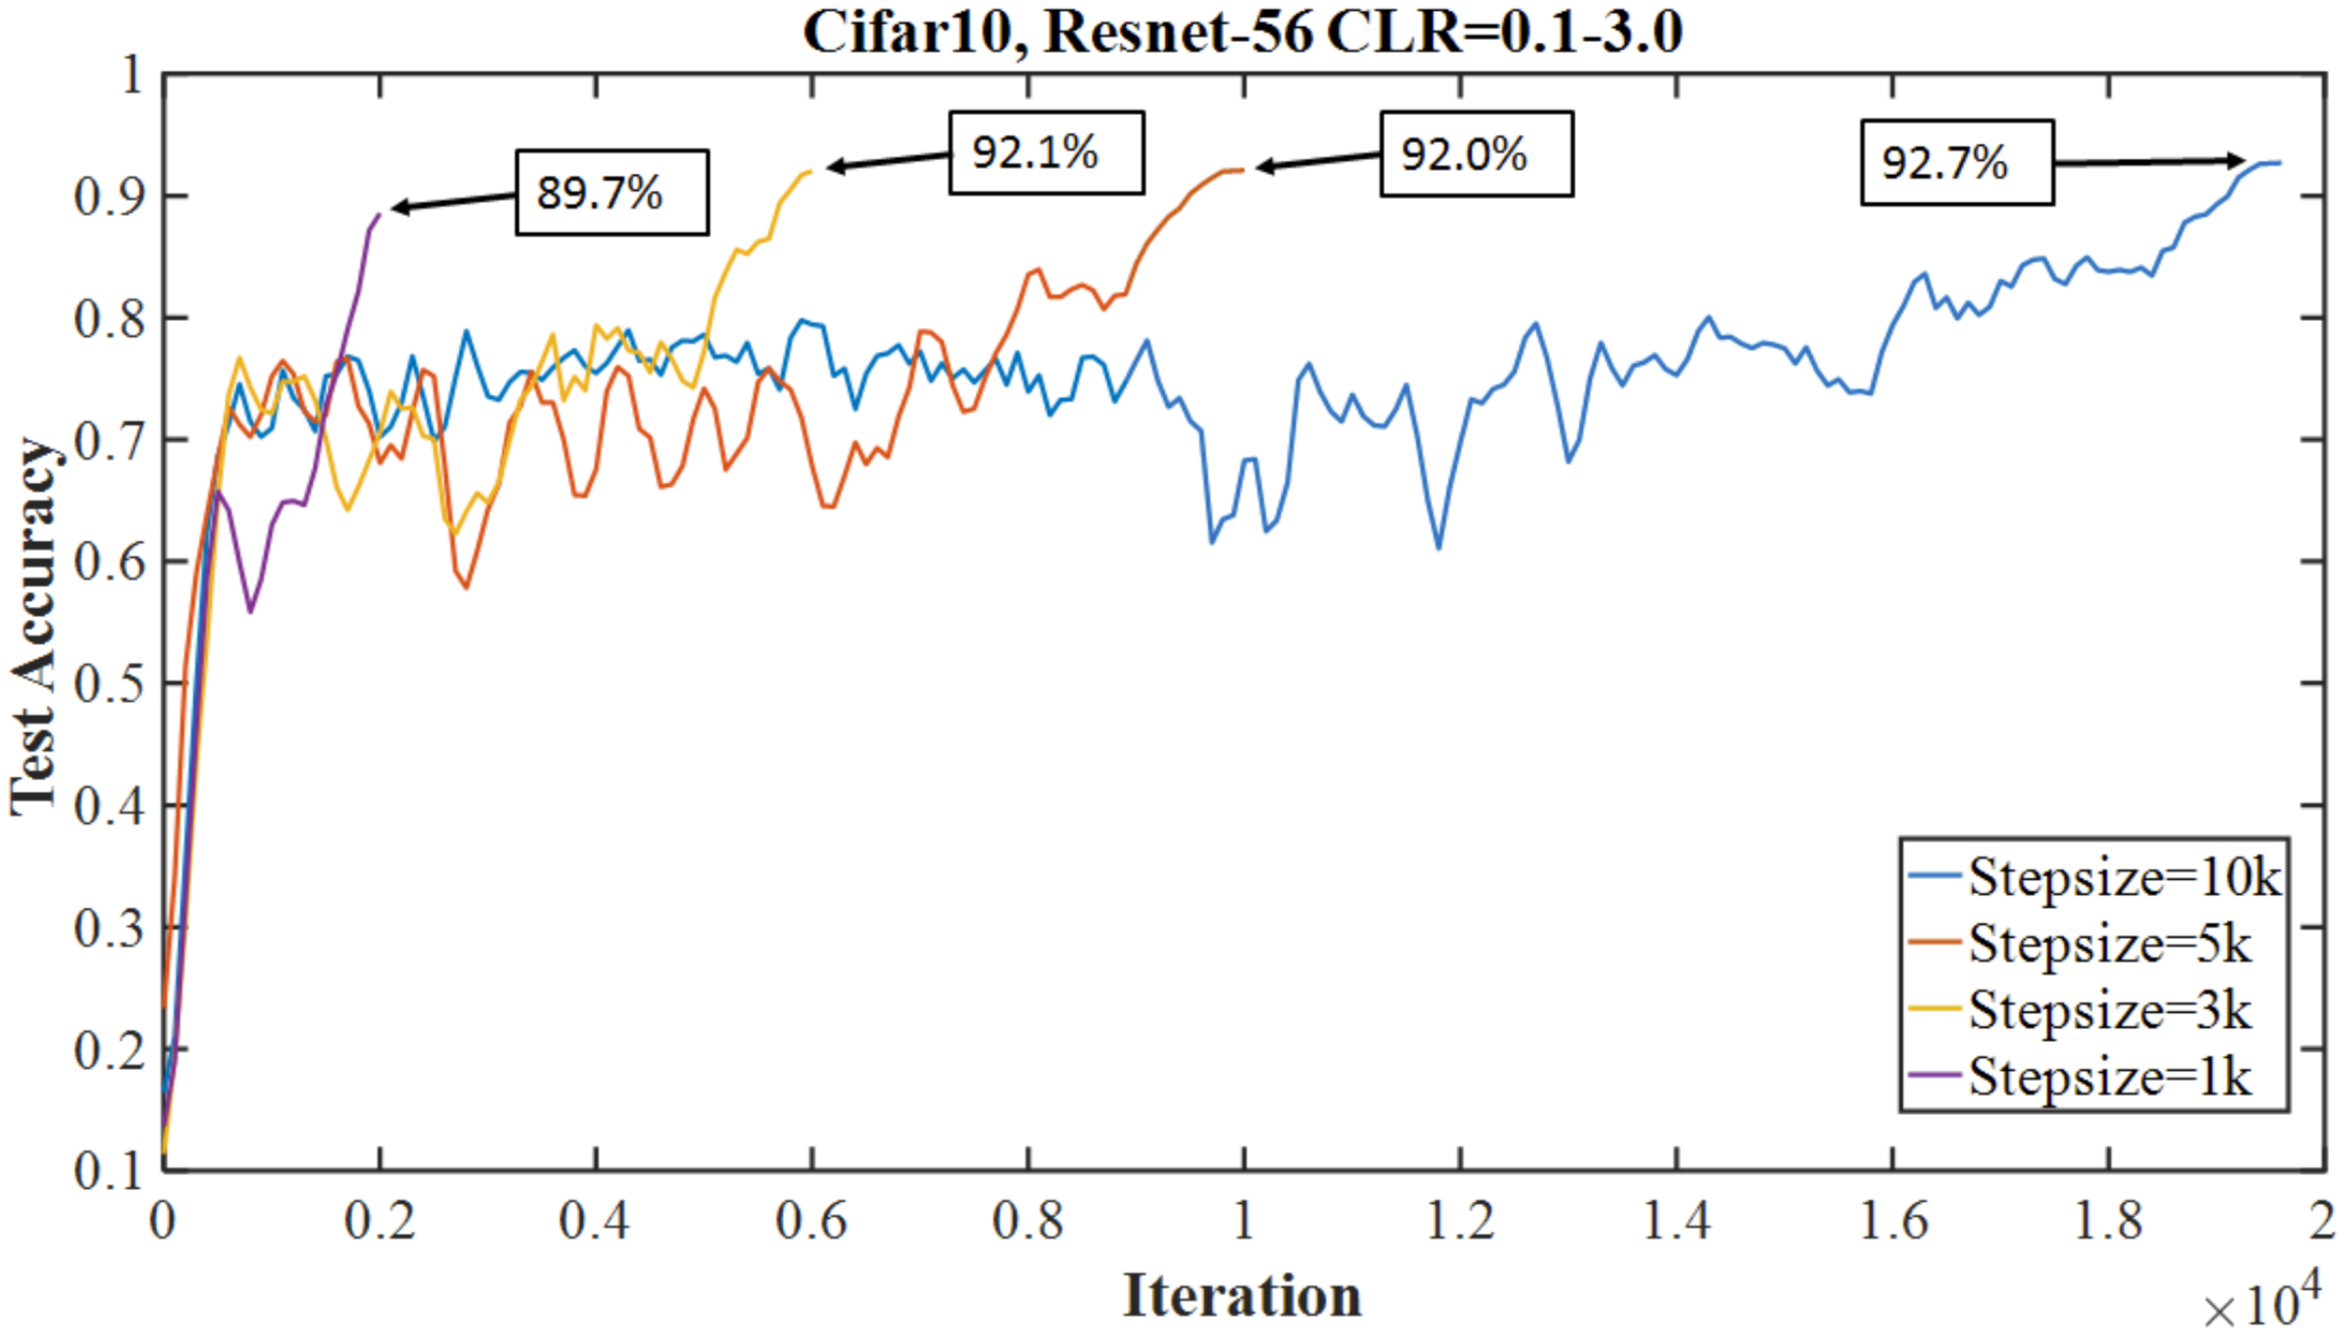
\includegraphics[trim=0 0 0 0, clip,
            width=3.25in]{images/figure_1b.png} &
        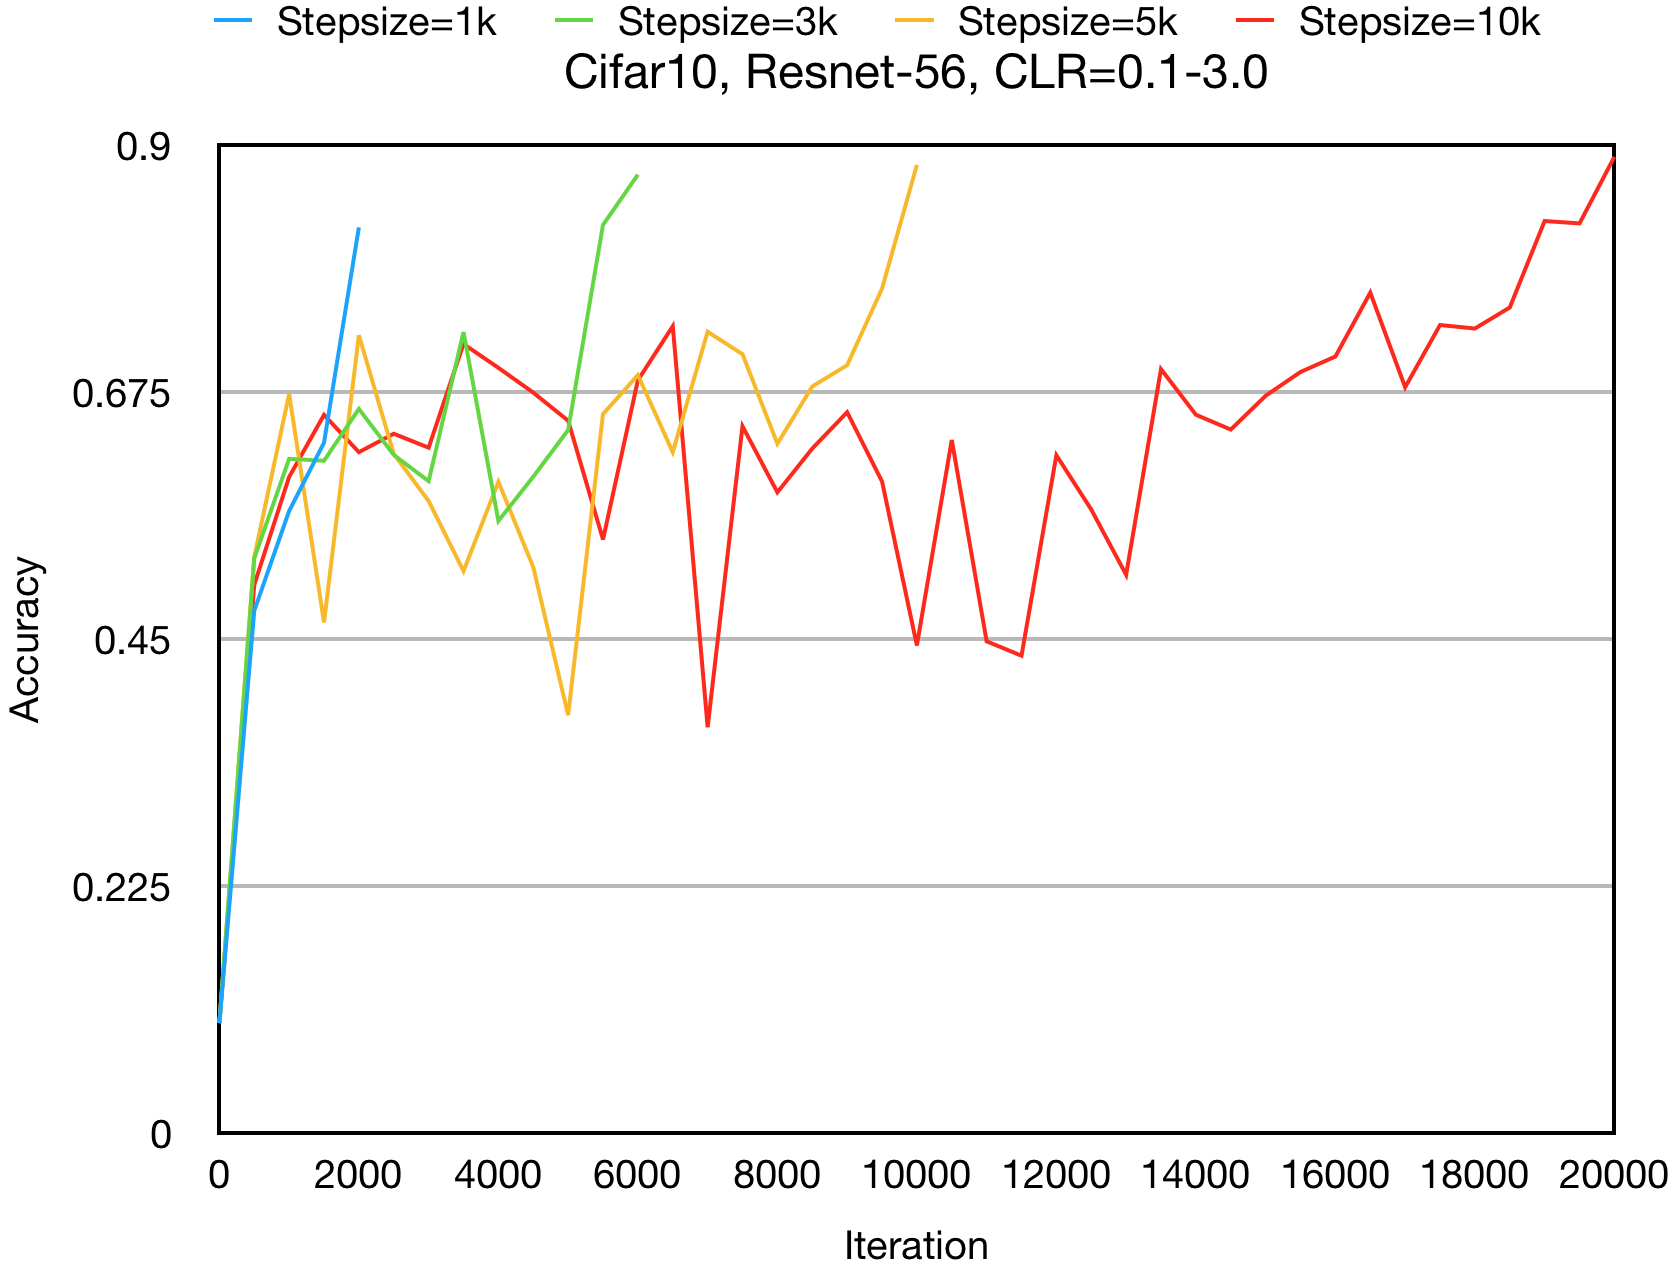
\includegraphics[trim=0 0 0 0, clip,
            width=3.25in]{images/step_sizes.png} \\
        Author's Results & Our Results \\
    \end{tabular}
    \caption{The effect of CLR step size on super-convergence.}
    \label{fig:step_size}
\end{figure*}

\subsection{Reduced Training Set}
One of the most appealing effects of super-convergence via the usage of CLR is
the increased performance with smaller training sets. This experiment,
displayed in figure \ref{fig:reduced_training_set} had the most contradicting
results with what the authors reported. While we got similar results with the
CLR tests, with both the ten and twenty thousand samples peaking towards the
end of their run, both of our PCLR tests peaked much faster than in the
authors' results. The PCLR test with ten thousand samples peaked before the CLR
runs, and the PCLR test with twenty thousand samples achieved higher test
accuracy with just a few thousand more iterations than the CLR runs.

\begin{figure*}[ht!]
    \begin{tabular}{cc}
        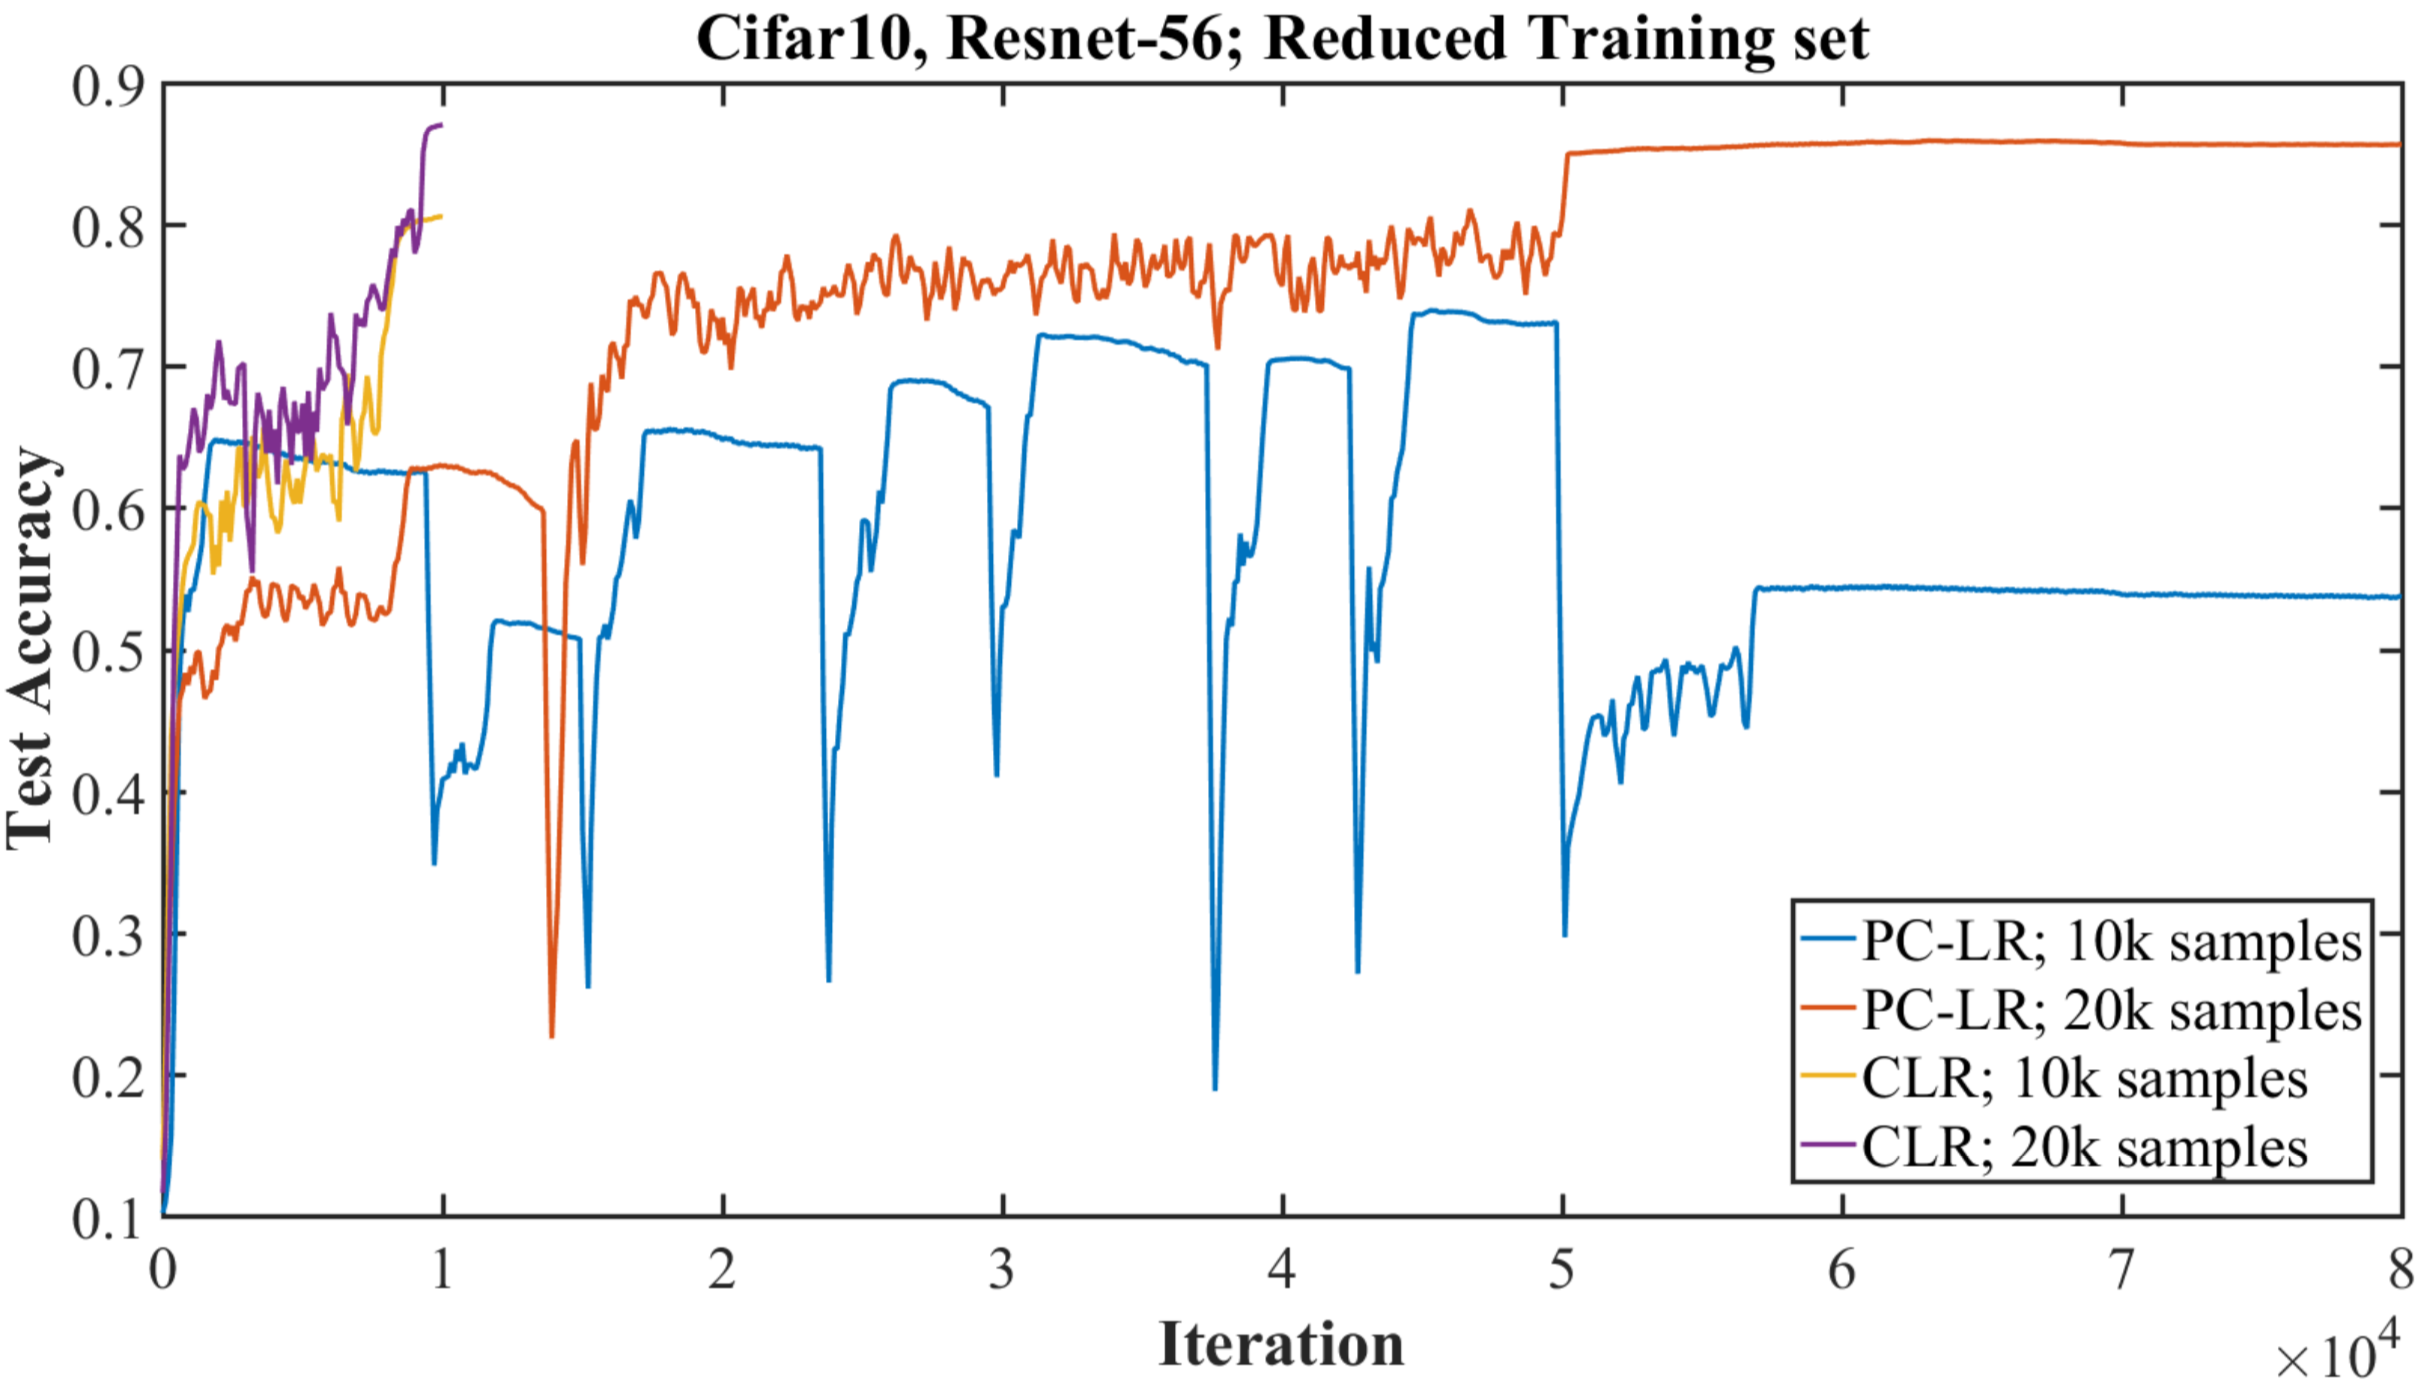
\includegraphics[trim=0 0 0 0, clip,
            width=3.25in]{images/figure_6a.png} &
        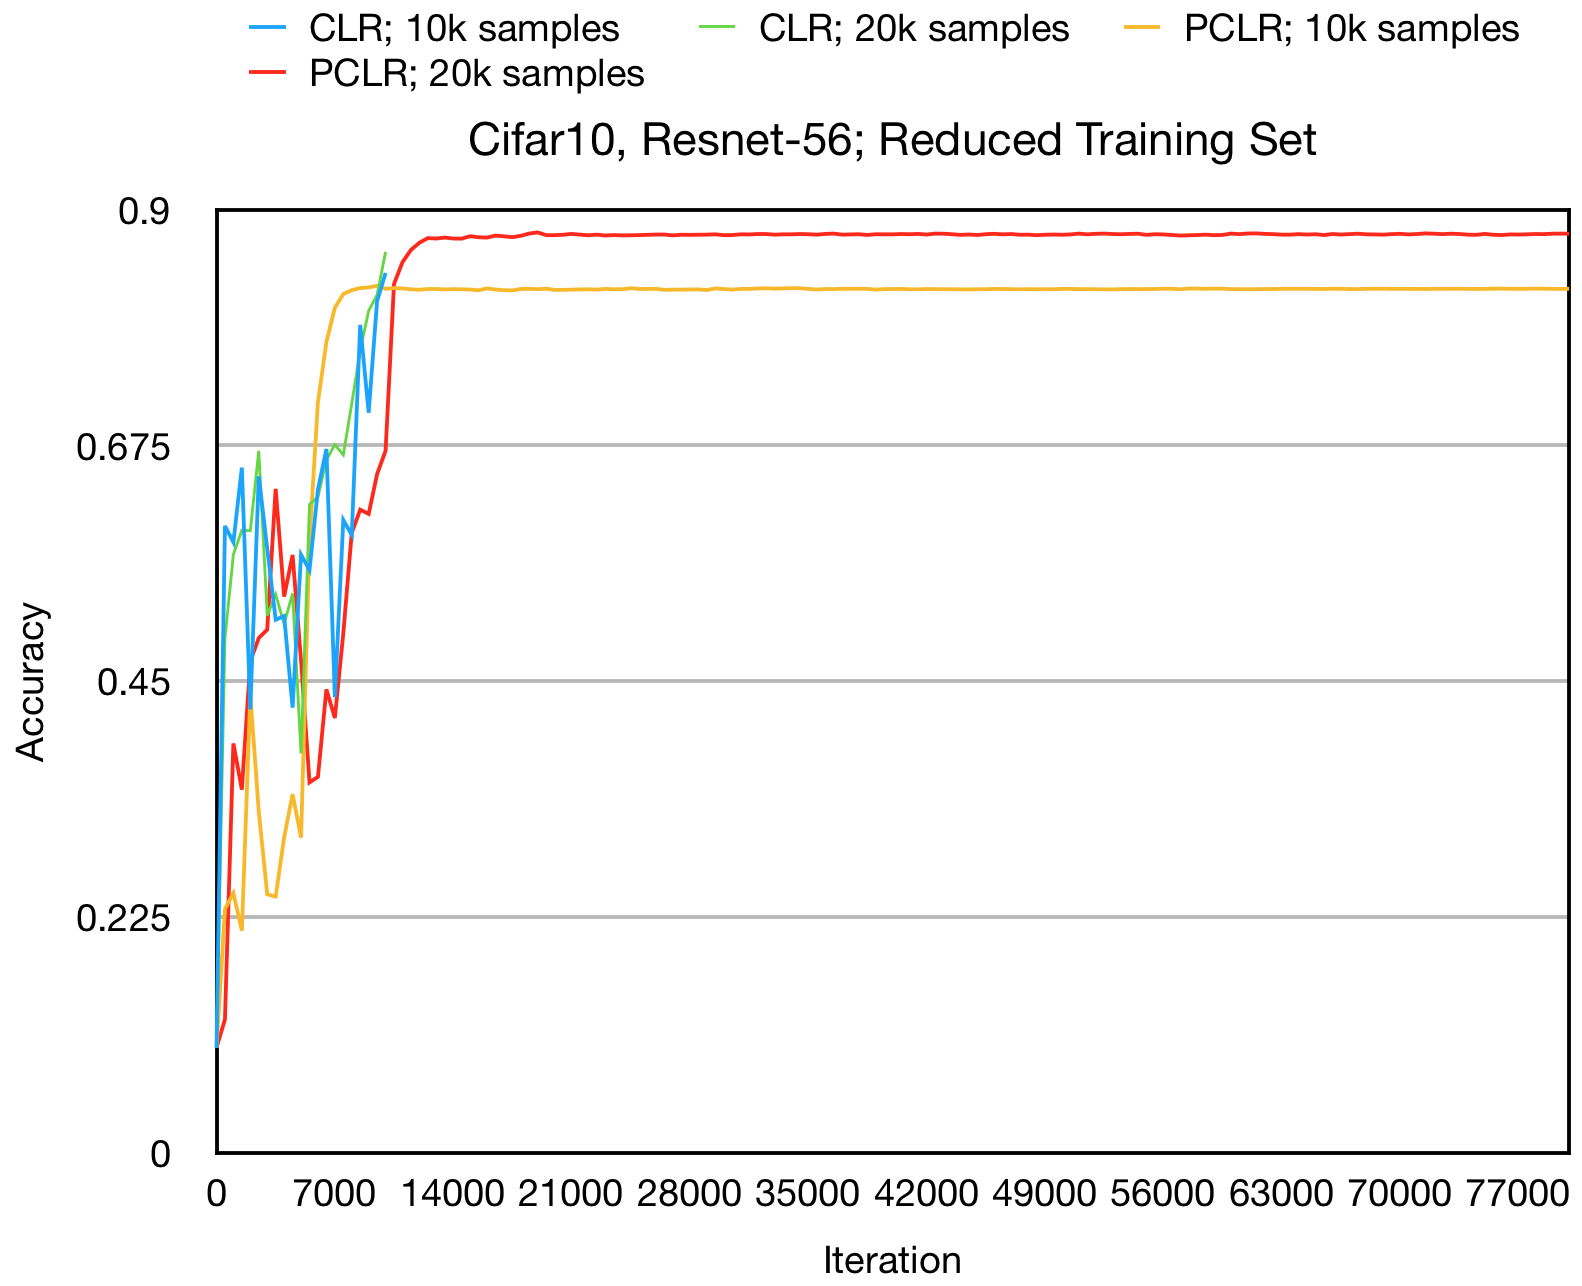
\includegraphics[trim=0 0 0 0, clip,
            width=3.25in]{images/reduced_training_set.png} \\
        Author's Results & Our Results \\
    \end{tabular}
    \caption{Reduced training set effect of PCLR and CLR.}
    \label{fig:reduced_training_set}
\end{figure*}

\subsection{ResNet Depth}
Here we attempt to reproduce the ResNet depth experiments, with results
displayed in figure \ref{fig:resnet_sizes}. Here, the authors' results are
consistent with intuition and their previous results. CLR peaks early and about
as high or higher than PCLR, and deeper architectures exhibit smaller test
error. Our results too display that deeper architectures work better on both
CLR and PCLR. However, consistent with our other results, we show that CLR
achieves worse final test error than PCLR.

\begin{figure*}[ht!]
    \begin{tabular}{cc}
        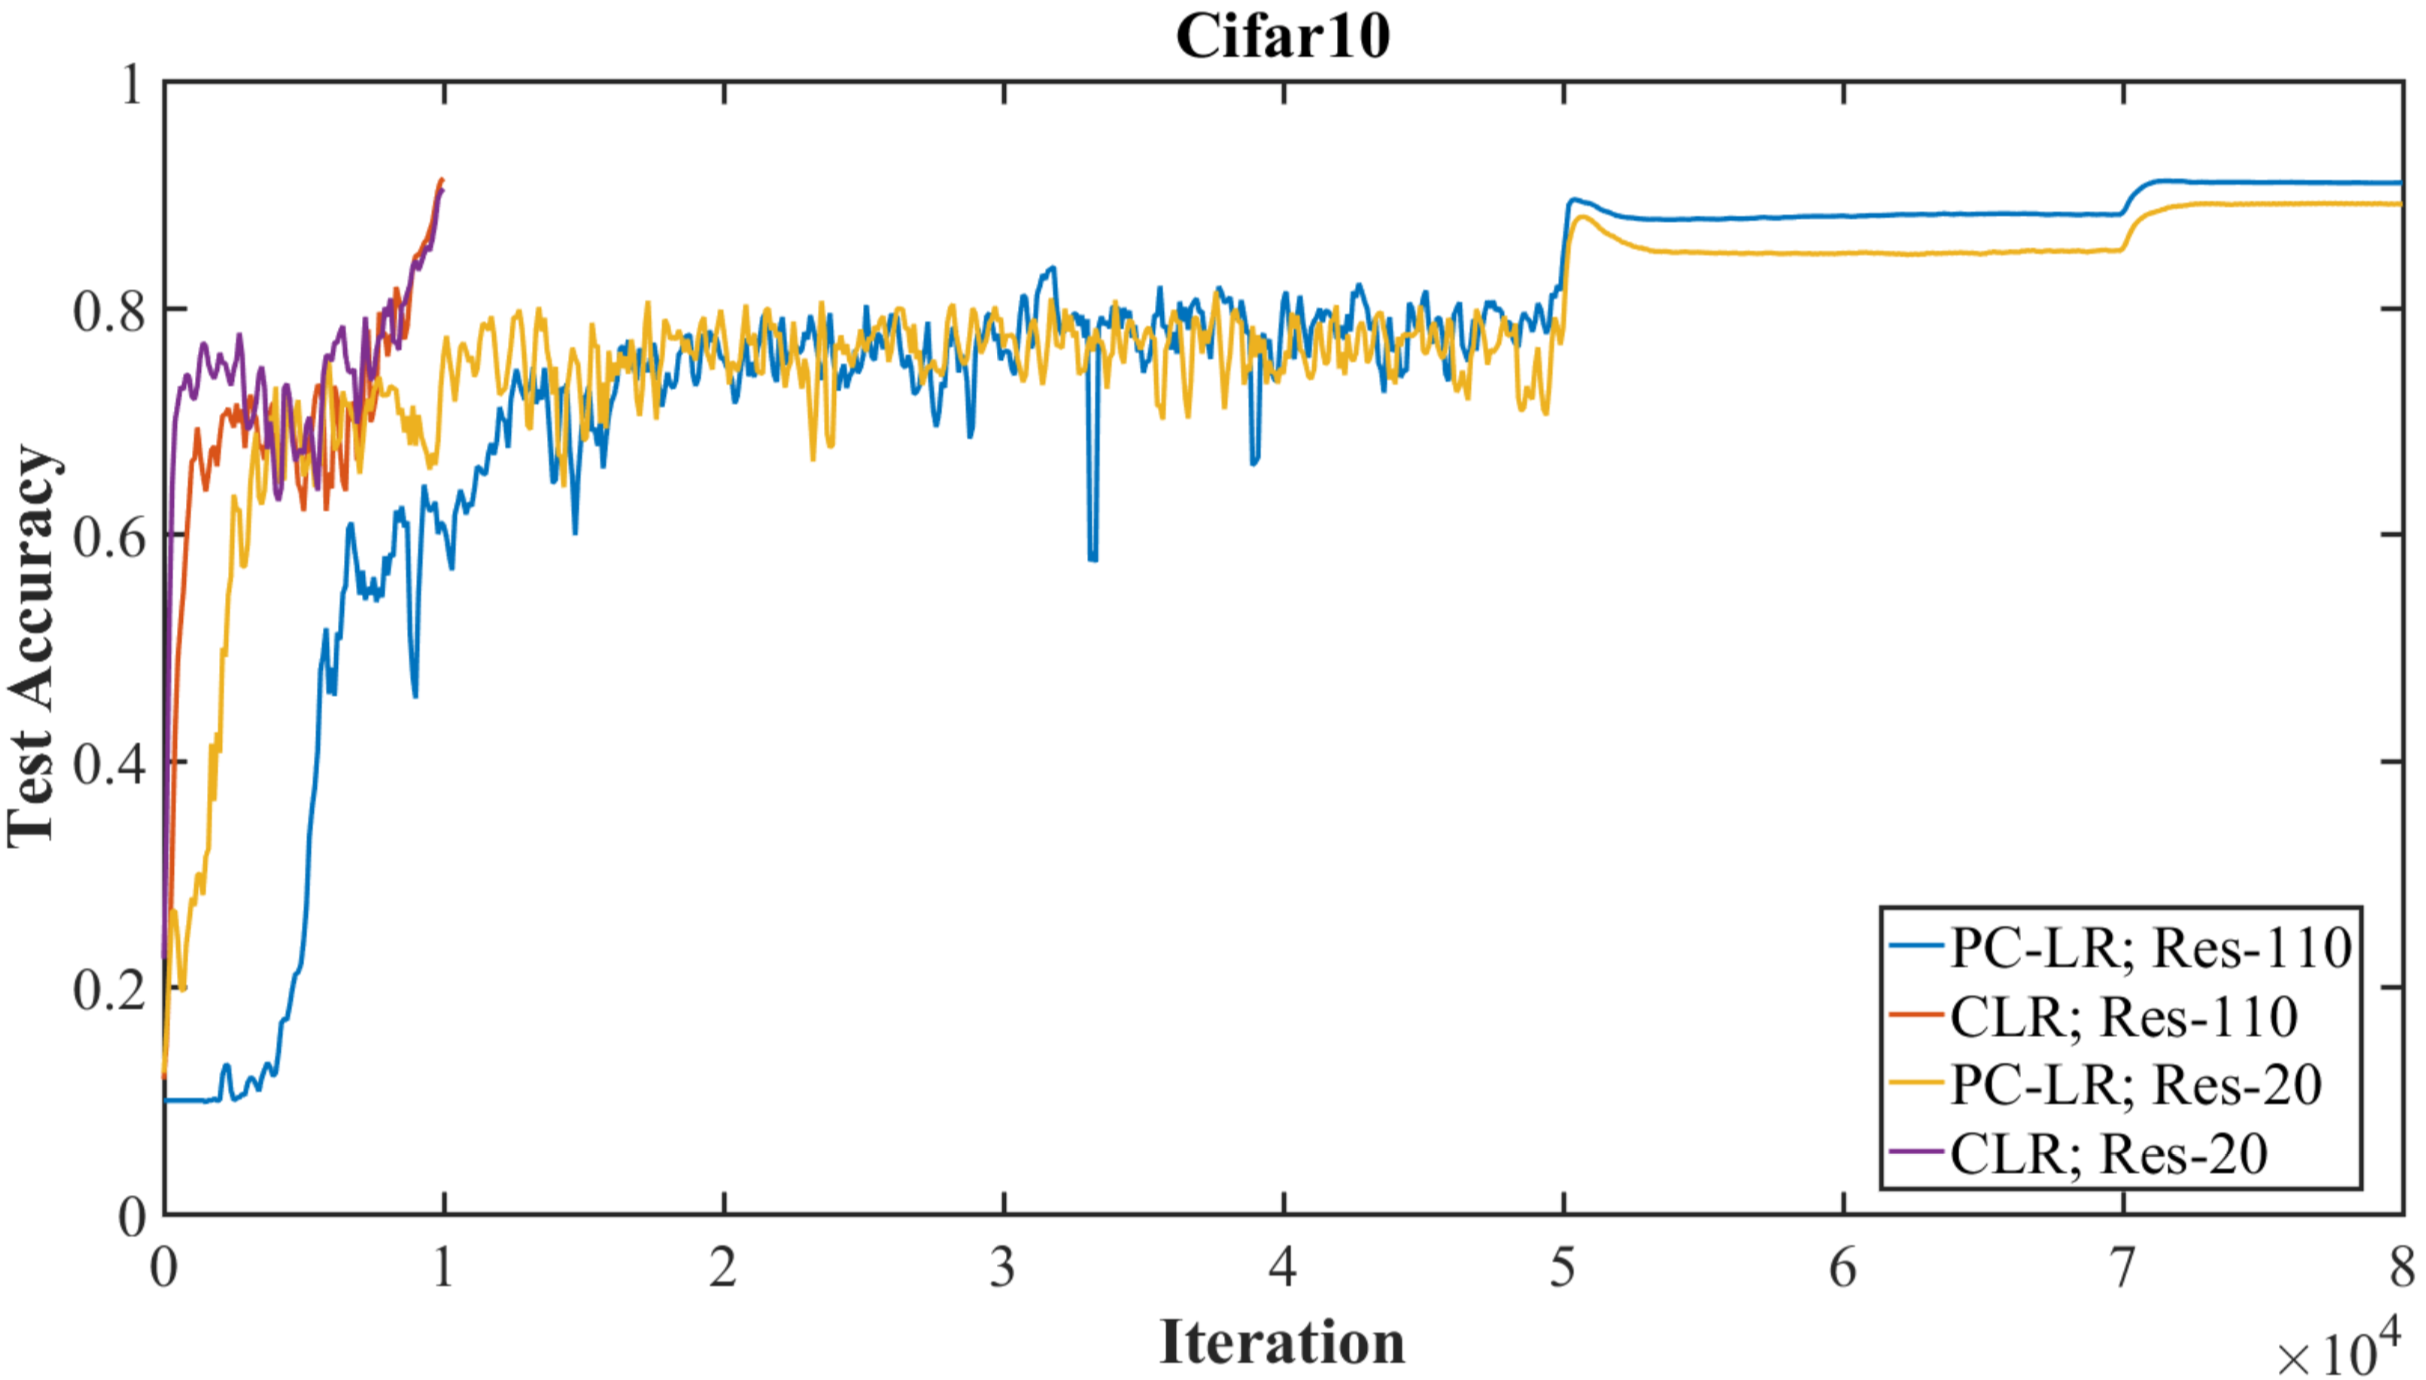
\includegraphics[trim=0 0 0 0, clip,
            width=3.25in]{images/figure_6b.png} &
        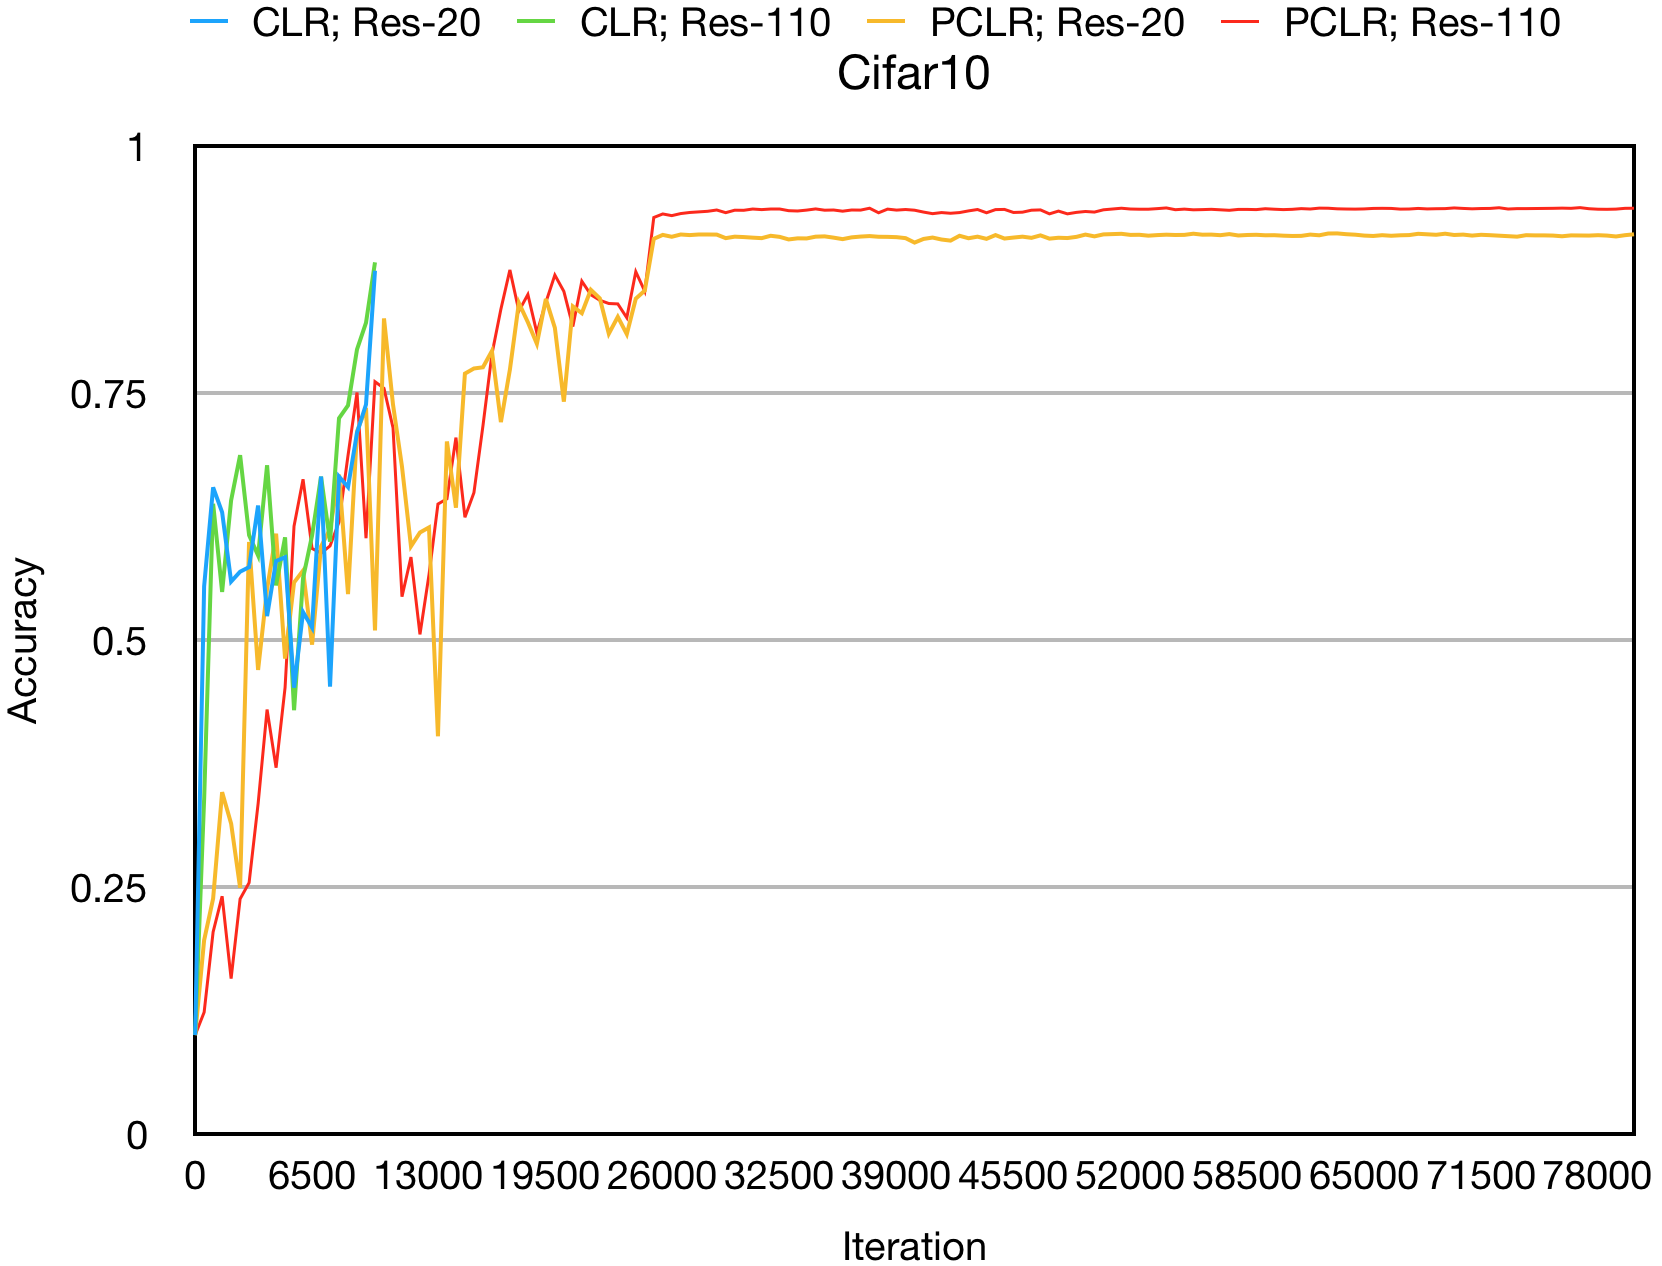
\includegraphics[trim=0 0 0 0, clip,
            width=3.25in]{images/resnet_sizes.png} \\
        Author's Results & Our Results \\
    \end{tabular}
    \caption{Effect of ResNet depth on CLR and PCLR.}
    \label{fig:resnet_sizes}
\end{figure*}

\subsection{CLR Min and Max Values}
Figure \ref{fig:table} displays results from previous tests as well as tests
for the min/max learning rate values for CLR. While we find that the range
$0.1-3.0$ works best for the learning rate, there does not appear to be a
consistent decreasing trend as the range is decreased.

CLR may turn out to be a dead-end research path in the near future. In
\cite{SGD_Minima} Jastrebski et al. show another way to help the network
generalize. By increasing the ratio of the learning rate to the batch size,
more noise is injected into the system during training which helps with
regularization. This appears to be happening in the super-convergence authors'
results. However, we expected to see a peak in CLR test results with smaller
learning rates in our test results since we are using smaller batch sizes. This
would keep the learning rate to batch size ratio more consistent with the
authors'. We did not see this behavior in our testing, possible indicating that
this ratio exhibits a non-linear relationship with testing accuracy.

\begin{figure*}[ht!]
    \begin{tabular}{cc}
        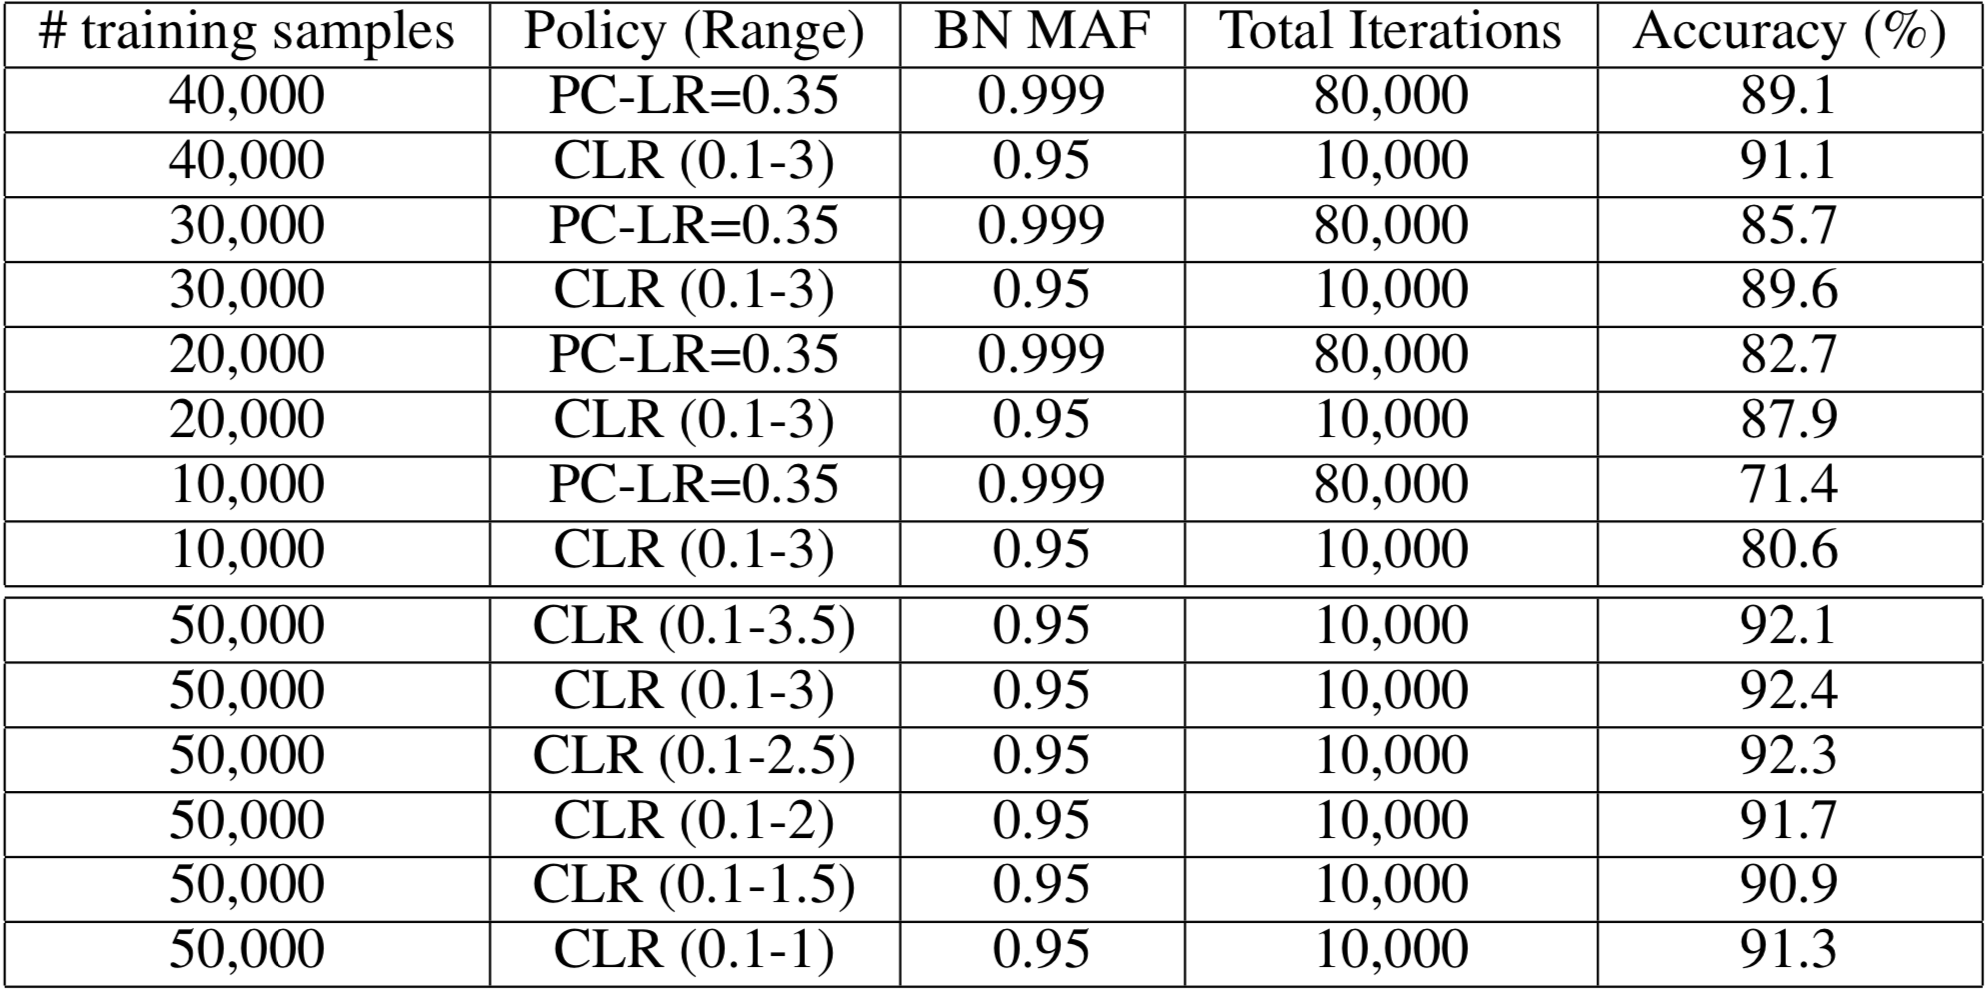
\includegraphics[trim=0 0 0 0, clip,
            width=3.25in]{images/their_table.png} &
        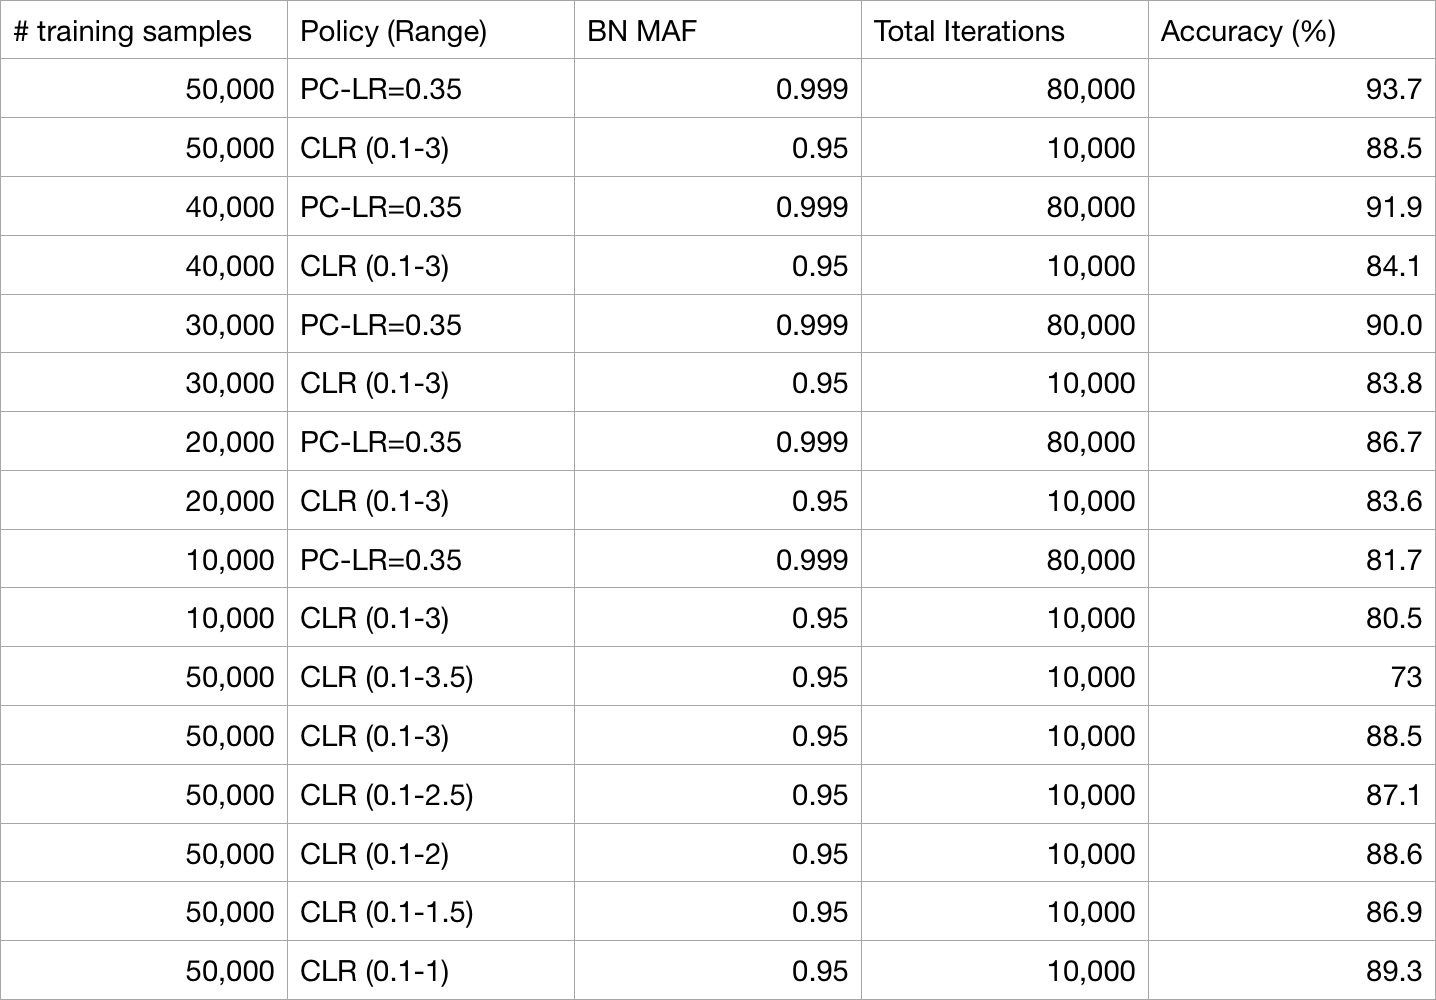
\includegraphics[trim=0 0 0 0, clip,
            width=3.25in]{images/our_table.png} \\
        Author's Results & Our Results \\
    \end{tabular}
    \caption{Full experimental results. Includes testing learning rate min/max values for CLR.}
    \label{fig:table}
\end{figure*}

%------------------------------------------------------------------------------

\section{Conclusion}
\label{sec:conclusion}
Overall we achieve similar but less pronounced results to the authors in our
training. We do find that ResNets can be trained on Cifar 10 and 100 using
large, cyclical learning rates faster than piecewise-constant learning rates by
nature of training ending early when using CLR.  Unlike the authors, however,
we find that the accuracy achieved using this method is below that of using a
piecewise-constant learning rate. In addition, we find that the CLR method is
not superior to the PCLR method when limited training data is used, contrary to
the authors' experiments. When adjusting step-size, learning rate range, and
number of iterations, we observe trends similar to those of the authors.

The discrepancy in peak accuracy between our super-convergence experiments and
those of the authors may be attributable to the very large batch size of 1000
used by the authors. This large batch size allows the authors to train their
network more quickly than we could, as we do not possess the hardware to use
such a large batch size. However, the general trends should and do still hold.

We believe that circumstances under which super-convergence occurs are too
limited to be considered useful and surmise that further investigation into the
benefits of large and cyclical learning rates rather than trying to reproduce
may be an isolated phenomenon under different circumstances.

\subsection{Cost of Reproduction}
What cost in terms of resources (computation, time, people, development effort,
communication with the authors).

Talk about how this method isn't very useful because it only works on: Cifar,
ResNets, large batch sizes. Discuss the impact of the paper (which is very
low).

{\small
\bibliographystyle{ieee}
\bibliography{bib}
}

\end{document}
